\documentclass [a4paper,11pt,utf8]{report}
\usepackage [francais]{babel}
\usepackage[utf8]{inputenc}
\usepackage[T1]{fontenc}
\usepackage{url}
\usepackage{graphicx}
\usepackage{color}

\setcounter{tocdepth}{3} % afficher les subsubsection dans la tableofcontents

\begin{document}
\begin{titlepage}
\begin{center}
{\bf Université Sciences et Technologies - Bordeaux 1} \vspace{0.5cm}\\

{\bf {\large Master 1 Informatique}}\\
{ \emph{Projet de programmation}}\\\vspace{5cm}



{\huge{\bf Génération procédurale de terrains et de planètes}}\\\vspace{1cm}

{\large{\bf{Rapport du 04 mars 2014 :}}}\vspace{1cm}

{\large\bf\it\rm Analyse des besoins et spécification des exigences (version 2.0)
}\vspace{2cm}


\end{center}


\hspace{1cm}\textbf{Réalisé par :}

\hspace{1cm}{Simon CAULE}

\hspace{1cm}{Pierre HUCHANT}

\hspace{1cm}{Solène JOLLY}

\hspace{1cm}{Adrien LAMOUREUX}\\


\hspace{1cm}\textbf{Encadrés par :} Adrien BOUSSICAULT\\

\hspace{1cm}\textbf{Client :} Emmanuel FLEURY\\

\end{titlepage}

\tableofcontents

\chapter*{Résumé}
La génération automatique de terrains virtuels est un problème sur lequel
planchent souvent les graphistes et les games designers, car pouvoir créer
 un monde virtuel persistant est une brique de base à de nombreuses
applications. Mais, même si le sujet a été maintes fois traité, il reste un
problème difficile non seulement techniquement à cause de la masse de calculs
 que cela représente mais aussi parce que le rendu final du paysage doit
paraître un tant soit peu réaliste aux yeux des utilisateurs.\\

Le but de ce projet est de créer une bibliothèque permettant la création de
terrains virtuels à partir de méthodes fractales. L'utilisateur de la bibliothèque
pourra réaliser des cartes carrées ou sphériques et disposera d'un choix
conséquent d'algorithmes de génération qui seront détaillés dans ce rapport.
La bibliothèque permettra aussi la visualisation des terrains avec différents
niveaux de détails.\\

Ce cahier des charges se compose de trois chapitres : les besoins fonctionnels, les besoins non fonctionnels et l'étude de faisabilité.

\chapter*{Objectifs}
La génération procédurale de terrains étant un sujet large, nous avons réalisé des choix d'implémentation.

\section*{Génération de terrains}
La génération procédurale de terrains est le fait de créer des terrains à l'aide d'algorithmes, sans interactions avec l'utilisateur. Nous avons choisi de réaliser une bibliothèque qui permettra à un utilisateur de générer facilement un terrain. Pour cela, la bibliothèque proposera des méthodes de génération de terrains carrés ou sphériques. Ces méthodes fourniront des terrains aussi réalistes que possible.

\section*{Interopérabilité entre la bibliothèque et certains visualisateurs existants}
Il existe de nombreux visualisateurs capables de créer un terrain à partir de cartes d'élévations et / ou de modèles externes.
Ainsi il sera intéressant de combiner le réalisme des cartes d'élévations et des modèles générés avec le rendu proposé par ces visualisateurs. Ceux choisis sont TerraGen3 (référence pour le travail de terrains) et Blender3D (open-source et très efficace pour le travail de modèles). Les terrains pourront également être importés.

\section*{Visualisateur intégré à la bibliothèque}

Le projet proposera également un visualisateur (vue et zoom sur le terrain). Toutefois, la conception de ce dernier ne sera pas prioritaire.

\section*{Scénario d'exécution}
La figure ci-après présente un scénario d'utilisation de notre
bibliothèque.
L'utilisateur spécifie les paramètres qu'il souhaite aux différentes composantes de
celle-ci. Effectivement, il aura accès aux principales structures (carte d'élévation,
grille, etc).
Les modules de la bibliothèque pourront être utilisés de façon indépendante même s'il
est évident que certains modules doivent être utilisés avant d'autres (e.g : création du terrain avant visualisation).


\begin{figure}[!ht]
    \begin{center}
        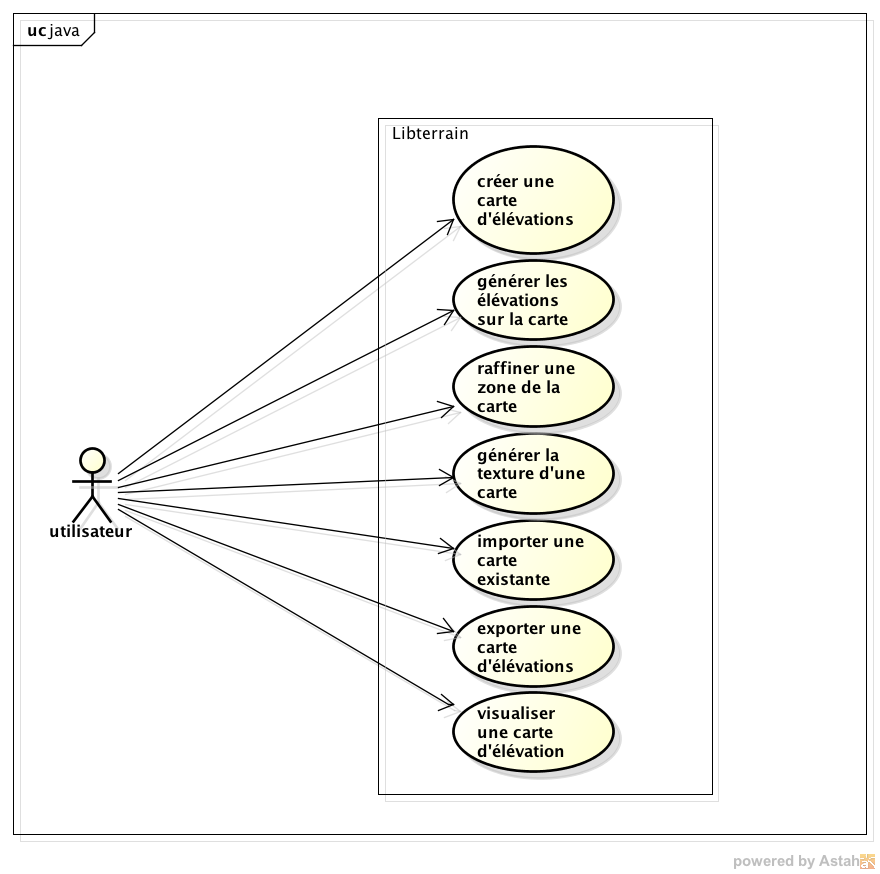
\includegraphics[width=15cm]{resources/use-case.png}
        \label{fig:use_case}
        \caption{Scénario d'exécution}
    \end{center}
\end{figure}


%Pour éviter la numérotation du sommaire
\thispagestyle{empty}

%%terragen :  Donc, un fois que nous aurons généré une carte à l'aide de notre bibliothèque, nous devrons réaliser une conversion au format .TER afin qu'elle soit compatible avec terragen.


\chapter{Besoins fonctionnels}

\section{Besoins prioritaires}

Ces besoins sont ceux que nous nous engageons à implémenter.

\subsection{Structures de données}
La bibliothèque devra proposer deux types de cartes d'élévations :\\
\textbf{sphériques} et \textbf{carrées}.

\subsection{Génération d'un terrain}
\subsubsection{Algorithmes}
Pour permettre la génération d'un terrain, les méthodes suivantes devront pouvoir
 être appliquées sur les cartes d'élévation (les méthodes suivies de la mention [prioritaire] sont celles qui doivent \^etre implémentées en priorité) :\\

\noindent méthodes des fractales :
\begin{itemize}
\item diamond-square ; [prioritaire]
\item midpoint displacement ; [prioritaire]
\item fractional brownian motion ;
\item multi-fractal midpoint displacement.
\end{itemize}
méthodes des bruits :
\begin{itemize}
\item simple noise ;
\item cell noise ;
\item Perlin noise ; [prioritaire]
\item value noise.
\end{itemize}
raffinement par modèles :
\begin{itemize}
\item erosion model.
\end{itemize}

\subsubsection{Raffinement}
S'il souhaite raffiner une zone précise, l'utilisateur pourra la sélectionner (en passant ses coordonnées en paramètres) afin d'appliquer une des méthodes de raffinement (de son choix) sur cette seule zone.

%\subsubsection{Risque}
%Biaiser la cohérence du terrain au niveau de la bordure de la zone raffinée.

%\subsubsection{Parade}
%Proposer une zone de lissage autour de la frontière de la zone raffinée.

%\subsubsection{Validation}
%Stresser la bibliothèque en la soumettant à divers facteurs :
%\begin{itemize}
%\item variation des paramètres d'entrée des méthodes de générations procédurales de façon aléatoire ;
%\item diverses tailles de cartes sous différents niveaux de détails ;
%\item exécution sur diverses machines ayant des différences au niveau physique (RAM, CPU, etc).
%\end{itemize}

\subsubsection{Génération de texture}
Il devra être possible de donner une couleur différente à chaque point de la carte en
fonction de son élévation.

\subsection {Génération d'une grille}

Pour les cartes carrées et sphériques, il sera possible de choisir une grille carrée, triangulaire ou hexagonale.

\subsection{Importation / exportation}
Les cartes d'élévations pourront être importées et exportées sous forme
d'images (.png, .jpeg) afin d'être lisible par d'autres logiciels
tels que Terragen 3 ou Blender 3D. \newline
Les modèles sont exportés sous format .obj pour être lisible par Blender3D.
Une méthode sera donc conçue pour lire les fichiers importés et une autre pour les concevoir dans le cas d'un export. 

\section{Besoins non prioritaires}

\subsection{Implémentation d'un visualisateur 3D}
Génération d'une simple représentation de la carte par rapport à la
carte d'élévation d'origine et du modèle construit par la bibliothèque.

Implémentation d'un zoom pour pouvoir visualiser la carte avec différents niveaux
de détail.

\chapter{Besoins non fonctionnels}

\section{Comportement}

\subsection{Performances}
La génération de terrains n'étant pas faite en temps réel, aucune exigence
concernant la vitesse de calcul n'est spécifiée : la qualité du rendu prime sur
le temps d'exécution. Le temps de génération de nos terrains pourra donc \^etre conséquent (de quelques secondes à quelques minutes).\\

Il n'y a pas d'interactivité entre l'utilisateur et le programme pendant l'exécution de ce dernier (le programme peut donc s'exécuter en tâche de fond).\\

\subsection{Facilité d'utilisation}
La bibliothèque devra \^etre facile à prendre en main pour l'utilisateur (qui sera un développeur) et devra proposer un maximum d'algorithmes de génération de terrains (parmis ceux qui sont décrits dans les besoins fonctionnels).\\

Il s'agit de développer une bibliothèque et non un logiciel. L'utilisateur
de notre projet est donc un développeur. En conséquence il n'est pas demandé
d'implémenter d'interface graphique pour l'utilisation de la bibliothèque elle-m\^eme, l'utilisateur final pourra, s'il le souhaite, en créer une en s'appuyant sur les différents services proposés par notre bibliothèque.\\

\subsubsection{Contraintes}
Une documentation devra être livrée avec la bibliothèque.

\subsubsection{Validation}
Plusieurs programmes d'exemples illustrant l'utilisation de notre bibliothèque seront livrés.

\subsection{Portabilité}
La bibliothèque sera développée pour les plateformes Linux/x86 et devra utiliser
GNU Autotools comme système de construction.

\subsubsection{Contraintes}
Toute utilisation de bibliothèque devra \^etre justifiée afin d'éviter la prolifération des dépendances. La bibliothèque boost ne devra \^etre utilisée qu'en cas d'absolue nécessité.

\subsection{Persistance des données de la génération procédurale}
Les exécutions avec les mêmes paramètres (méthodes, graine aléatoire, etc)
doivent fournir le même résultat.

\subsubsection{Validation}
Pour N exécution d'une méthode avec des paramètres identiques, comparer les cartes d'élévations obtenues (sommet par sommet) en vérifiant que les sommets aient les mêmes élévations. 

\section{Besoins organisationnels}

\subsection{Standards, processus de développement}

\subsubsection{Langage}
L'implémentation sera faite en C++11, la version standard actuelle de C++ depuis
2011.

\subsubsection{Style de codage}
Le projet devra respecter le style de codage de linux :\\
\url{https://www.kernel.org/doc/Documentation/CodingStyle}\\
\emph{(Dernière visite : 10/02/2014)}
%\subsection{Gestion du temps}
%% TODO diagramme Gant

\section{Autres besoins}
\subsection{Contraintes légales}
Le projet sera distribué sous Licence Publique Générale Limitée GNU (GNU LGPL).

Nous avons choisi cette licence car c'est une licence de logiciel libre mais
moins contraignante que la GPL. En effet elle autorise à lier un programme
développé sous cette licence à du code non (L)GPL. Il sera donc possible d'utiliser notre bibliothèque dans un programme publié sous une autre licence sans révoquer celle-ci.

\subsection{Contraintes d'interopérabilité}
Les cartes d'élévation produites par notre bibliothèque devront être lisible par les visualisateurs
 suivants : TerraGen 3 et Blender 3D.\\
\textbf{Terragen 3} utilise des fichiers au format .TER et les modélise sous forme de terrains.\\
Pour \textbf{Blender 3D}, les traitements en amont sont plus simples car ce logiciel charge
une carte d'élévation (image en niveaux de gris) et sous forme de modèle (fichiers
.obj).
Les configurations se font ensuite depuis Blender 3D.


\chapter{Faisabilité}
\section{Estimation de la taille mémoire requise pour les cartes d'élévations}
La figure~\ref{fig:heightmap_memory} illustre la taille mémoire requise pour
stocker les cartes d'élévations en fonction de leurs tailles et du type des entiers
utilisés. Pour permettre plus de lisibilité le graphique utilise une échelle
logarithmique.\\

\begin{figure}[!ht]
    \begin{center}
        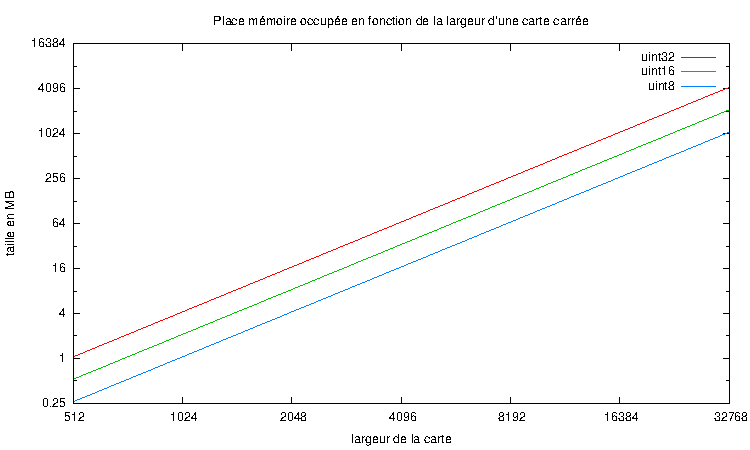
\includegraphics[width=15cm]{resources/heightmap-memory.pdf}
        \label{fig:heightmap_memory}
        \caption{taille mémoire occupée par une carte d'élévations}
    \end{center}
\end{figure}

\begin{itemize}
\item si l'on utilise des entiers non signés sur 8 bits (uint8), les valeurs
possibles pour les élévations s'étalent de 0 à 255, cet intervalle est assez
restrictif et limite la précision de la carte.

Cependant la place occupée en mémoire est faible (environ 256 Mo pour une carte
carrée de largeur 16 384) ;\\

\item si l'on utilise des entiers non signés sur 16 bits (uint16), les valeurs
possibles pour les élévations s'étalent de 0 à 65 535, cet intervalle est tout à
fait suffisant pour produire des carte ayant un niveau de détail élevé.

De plus la place occupée en mémoire est acceptable (environ 512 Mo pour une carte
carrée de largeur 16 384) ;\\

\item si l'on utilise des entiers non signés sur 32 bits (uint32), les valeurs
possibles pour les élévations s'étalent de 0 à 4 294 967 295, cet intervalle est
démesurément grand et n'est pas nécessaire pour produire des carte ayant un
niveau de détail élevé.

De plus la place occupée en mémoire est importante (environ 1 Go pour une carte
carrée de largeur 16 384).
\end{itemize}
%\chapter*{Conclusion}
La rédaction de ce cahier des charges nous a permis de définir et de nous approprier notre projet de programmation. En effet, nous avons fait des choix qui orienteront notre approche du projet au cours des semaines à venir.

%Pour éviter la numérotation du sommaire
\thispagestyle{empty}


\end{document}
